\chapter{Resultados e discussão}
\label{chap:resultados}

Para apresentação dos resultados encontrados ao longo da implantação da mesa cartesiana no 
laboratório de sistemas térmicos e uma posterior discussão, os temas foram divididos de acordo 
com a metodologia (seção \ref{ch:metodologia}). Primeiramente são apresentados os resultados do sistema mecânico, 
em seguida são mostrados os resultados da programação do sistema de software.

\section{Sistema mecânico}\label{sec:resmecanico}
    
A Figura \ref{fig:mesatunel} apresenta o esquema do sistema mecânico 
da mesa cartesiana dentro do túnel de vento. Assim, é possível observar que a estrutura da mesa 
cobre praticamente toda a seção transversal da área de teste. Permitindo assim uma medição automatizada com 
deslocamentos precisos tendo uma maior facilidade na obtenção dos dados, já que não é necessário desligar 
o túnel de vento e abrir a seção de testes a cada iteração. 

\begin{figure}[H]
\centering
\caption{Mesa cartesiana dentro do túnel de vento.}\label{fig:mesatunel}
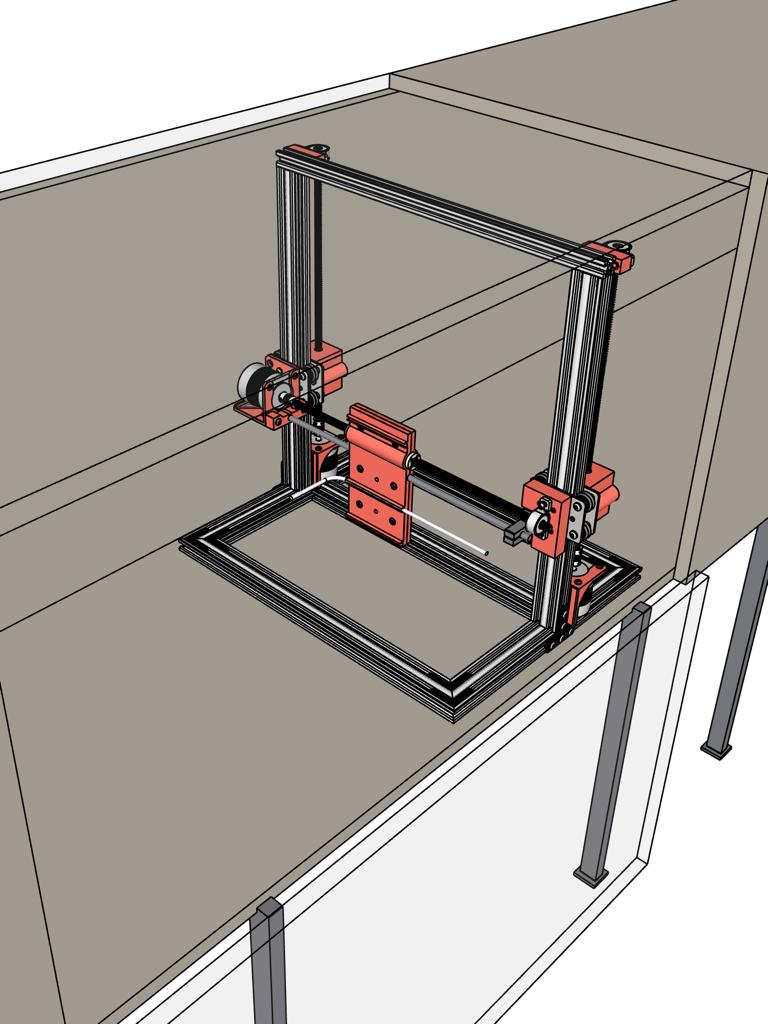
\includegraphics[scale = 0.35]{figuras/mesatunel}
\end{figure}

%PRECISA DE REFERENCIA PARA TABELA DA LISTA DE MATERIAIS
Para o desenvolvimento da mesa cartesiana foi necessário adquirir componentes estruturais e 
mecânicos de fornecedores, listado conforme a Tabela \ref{tab:listamateriais}, porém algumas peças terão 
que ser impressas, com filamento de \ac{PLA}, conhecido 
como \ac{PLA}, em impressora 3D. Essas peças serão discriminadas a seguir. 

As Figuras \ref{fig:mesacartesianaperfil} e \ref{fig:mesacartesianaperfiltraseira} mostram uma 
imagem da mesa cartesiana possibilitando uma melhor compreensão do funcionamento dos seus componentes.

\begin{figure}[H]
\centering
\caption{Sistema mecânico da mesa cartesiana vista de perfil.}\label{fig:mesacartesianaperfil}
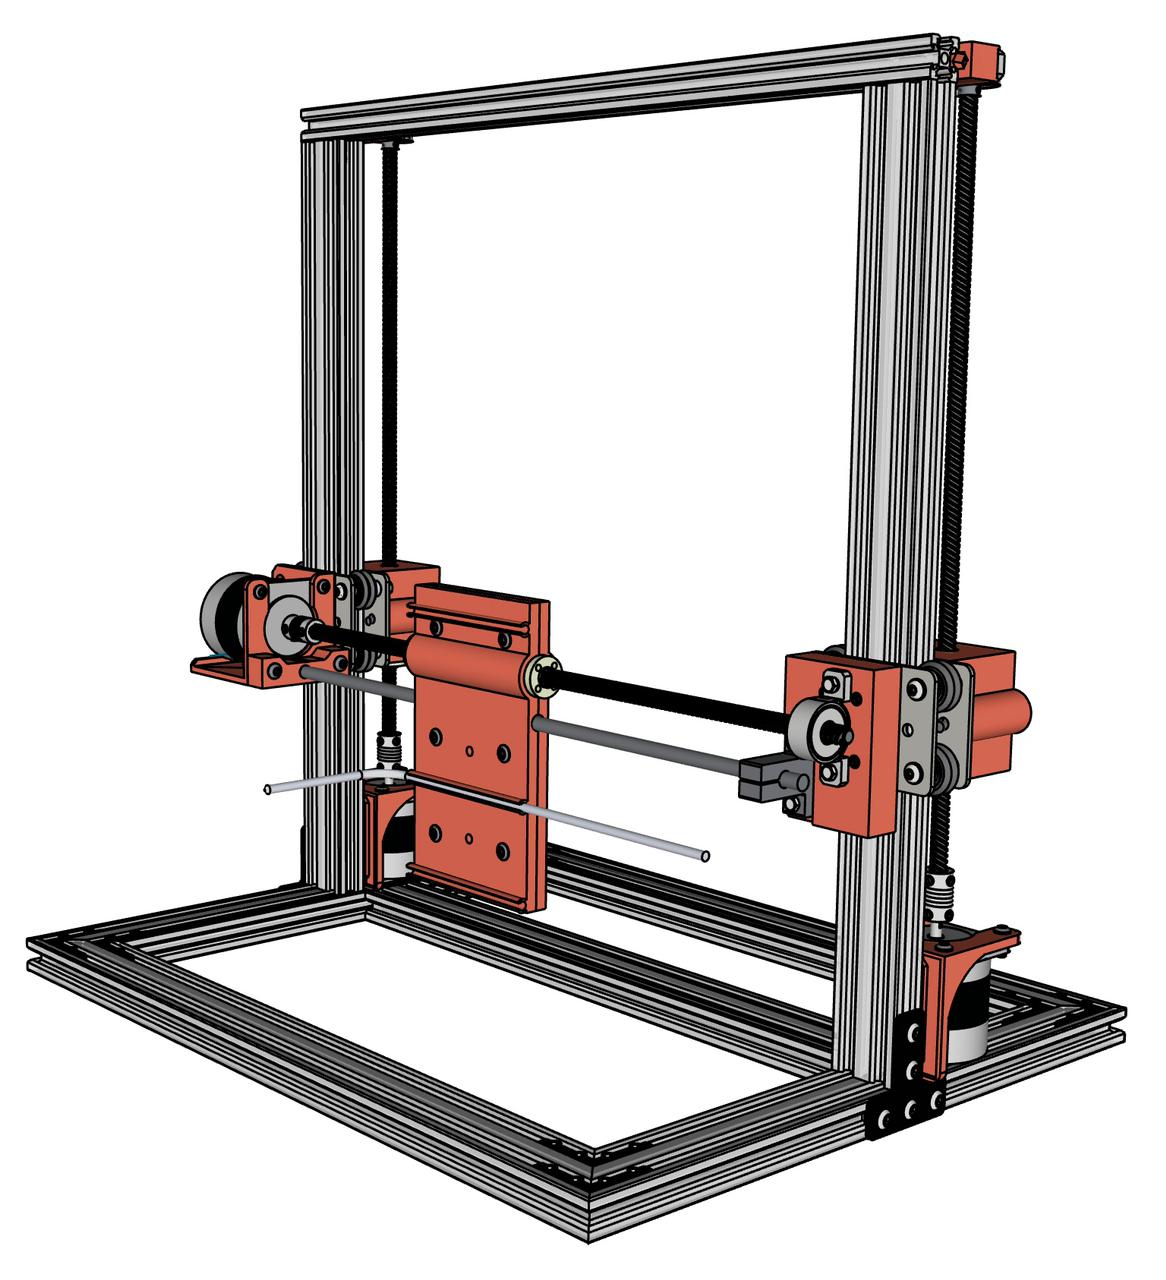
\includegraphics[scale = 0.35]{figuras/mesacartesianaperfil}
\end{figure}

\begin{figure}[H]
\centering
\caption{Sistema mecânico da mesa cartesiana vista de perfil traseira.}\label{fig:mesacartesianaperfiltraseira}
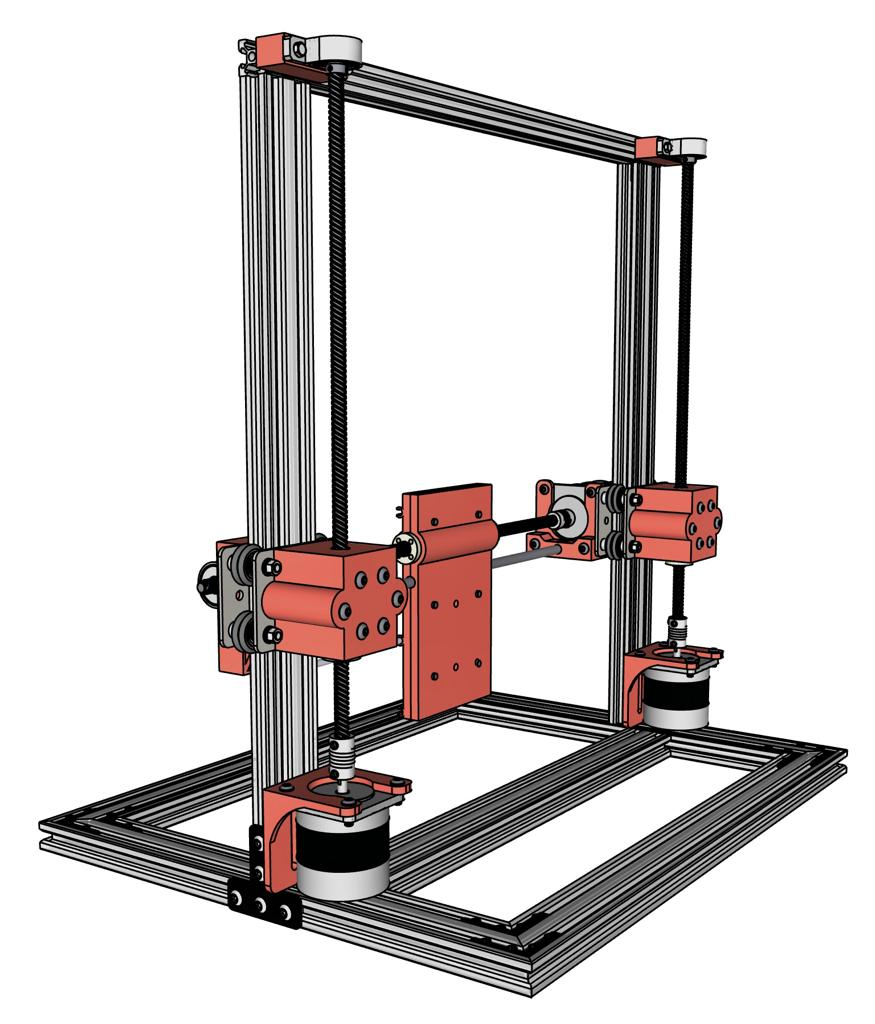
\includegraphics[scale = 0.35]{figuras/mesacartesianaperfiltraseira}
\end{figure}
                
Os elementos estruturais da mesa são em alumínio, para conferir-lhe uma considerável resistência, 
leveza e bom acabamento. Foram utilizados os perfil estrutural V-Slot 20~x~40~mm para compor a base 
e as laterais do pórtico e o perfil estrutural V-Slot 20~x~20~mm para a parte superior do pórtico. 
Para a união desses perfis foram utilizados, na base, conectores internos de 90°. Na união da 
base ao pórtico foi utilizado placa de conexão T fixada com parafusos Allen cabeça abaulada 
M6~x~10~mm e porca T reforçada com rosca M6. Já a união da parte superior do pórtico com suas laterais foi 
realizada com parafusos Allen cabeça abaulada M6~x~16~mm.

\pagebreak
Lista dos componentes em PLA:
\begin{itemize}
    \item 1 - Suporte do mancal;
    \item 2 - Suporte do motor de passo;
    \item 3 - Suporte de elevação;
    \item 4 - Suporte do motor horizontal;
    \item 5 - Suporte da haste e mancal;
    \item 6a - Suporte de serviço parte frontal;
    \item 6b - Suporte de serviço parte traseira;
\end{itemize}

Na Figura \ref{fig:vistaexplodida} são apresentados (em vista explodida) os suportes 
que devem ser fabricados em PLA.

\begin{figure}[H]
\centering
\caption{Vista explodida dos componentes em PLA.}\label{fig:vistaexplodida}
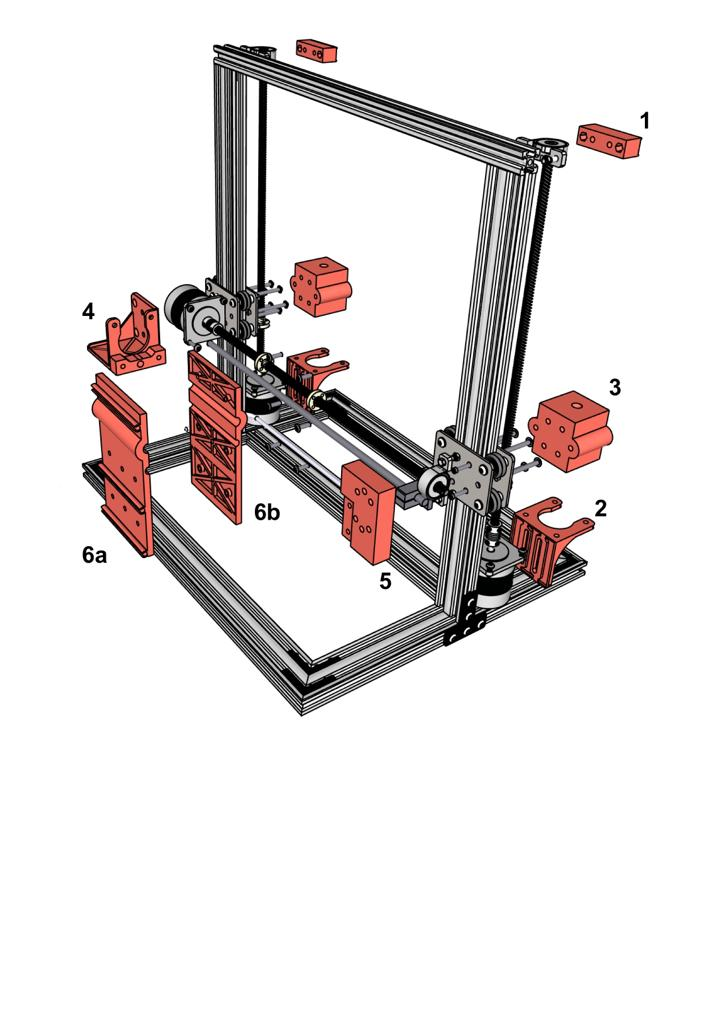
\includegraphics[scale = 0.45]{figuras/vistaexplodida}
\end{figure}

\pagebreak
%PRECISA DE REFERENCIA PARA FIGURA
Para o sistema de transmissão foram utilizados fusos TR8~x~8~mm unidos aos motores de passo 
por meio de acoplamento flexível em alumínio 5~x~8~mm e apoiados na outra extremidade por 
mancal de rolamento, para dar sustentação e mobilidade ao fuso. Para que se conseguisse 
a distância necessária da estrutura até o fuso e garantisse que este mantivesse a 
verticalidade, foi desenvolvido um suporte denominado de Suporte do Mancal, fabricado 
em \ac{PLA} conforme Figura \ref{fig:ressuportemancal}.

\begin{figure}[H]
\centering
\caption{Suporte do mancal.}\label{fig:ressuportemancal}
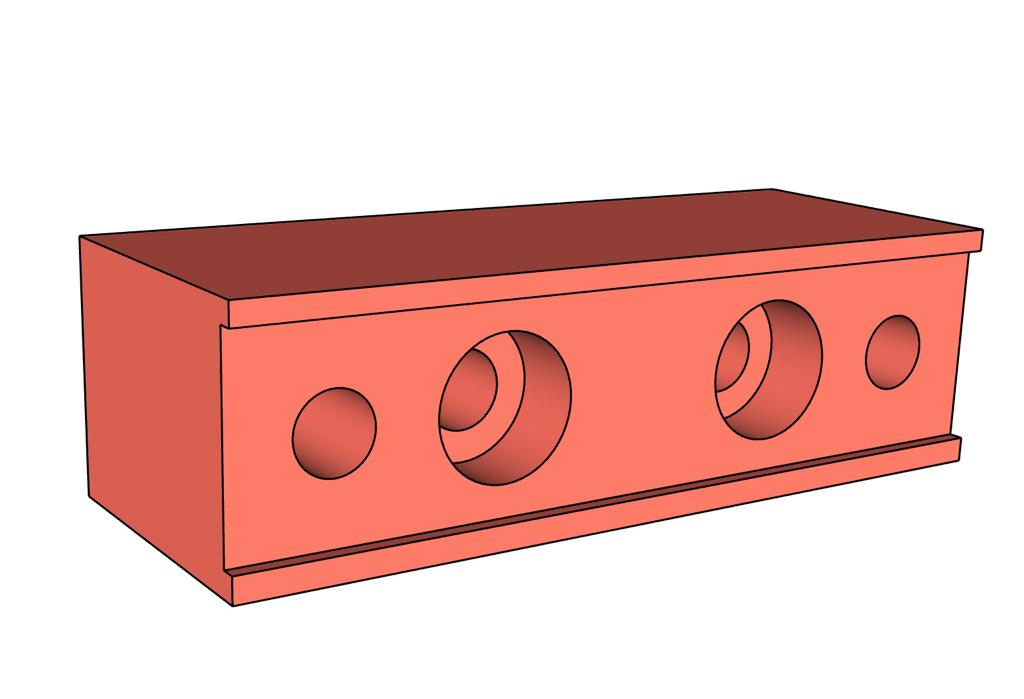
\includegraphics[scale = 0.4]{figuras/ressuportemancal}
\end{figure}
            
\pagebreak

Para fixação dos motores de passo dos eixos verticais, foi criado um suporte denominado 
de Suporte do Motor de Passo fabricado em \ac{PLA}. Este suporte deve ser preso à estrutura 
por meio de parafusos Allen de cabeça abaulada com rosca M6~x~10~mm e porcas T reforçadas com rosca M6, 
o motor de passo deve ser fixado após a fixação do suporte.

\begin{figure}[H]
\centering
\caption{Suporte do motor de passo.}\label{fig:ressuportemotorpasso}
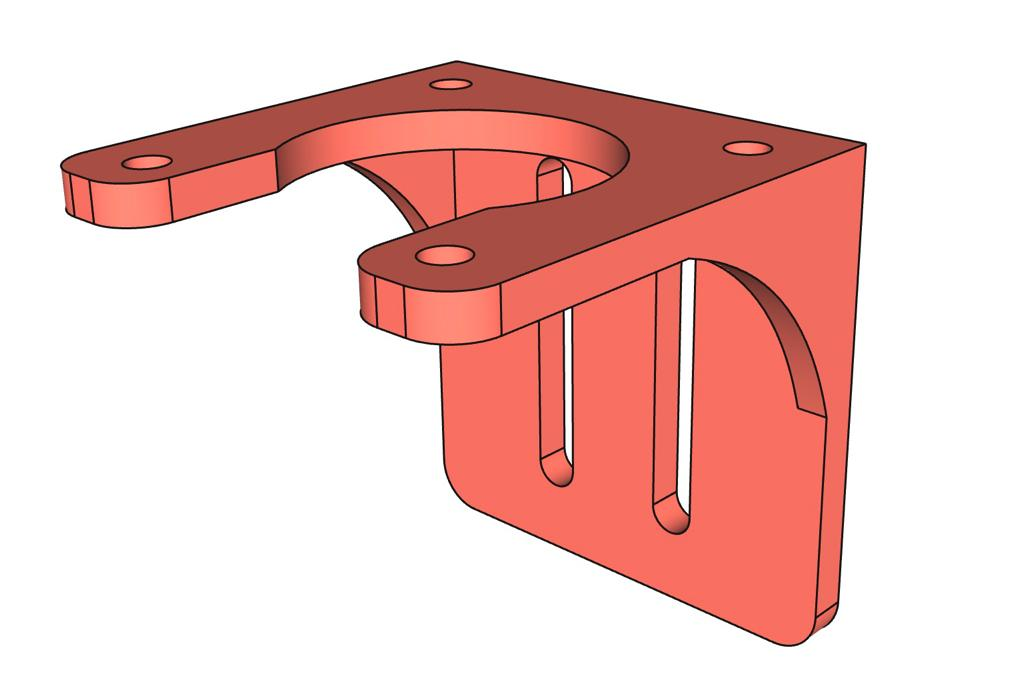
\includegraphics[scale = 0.4]{figuras/ressuportemotorpasso}
\end{figure}

\pagebreak

No sistema de elevação foram utilizados guias ajustáveis com roldanas para perfil 20~x~40~mm V-Slot 
com 4 apoios. Esses elementos são unidos ao fuso por meio de uma peça fabricada em \ac{PLA} 
denominada de Suporte de Elevação, conforme Figura \ref{fig:ressuporteelevacao}. Em cada um dos 
suportes foi instalado uma castanha em latão para fuso trapezoidal TR8~x8~mm de 4 entradas.

\begin{figure}[H]
\centering
\caption{Suporte de elevação.}\label{fig:ressuporteelevacao}
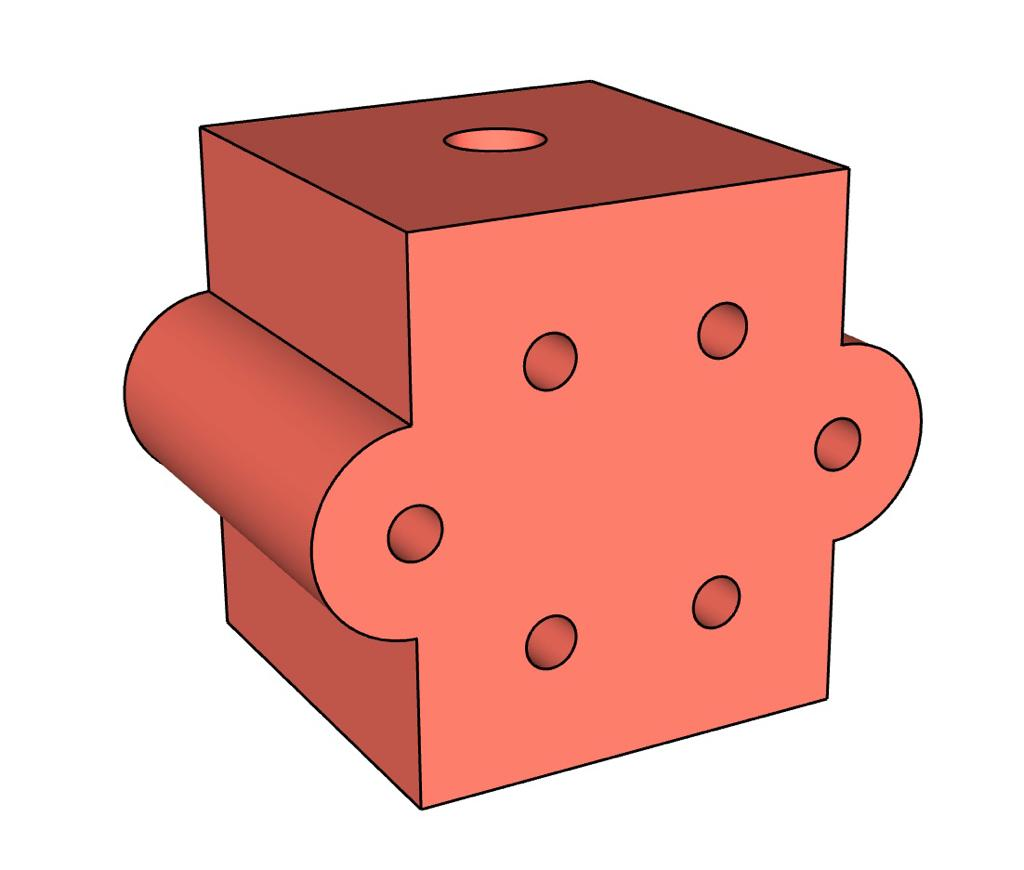
\includegraphics[scale = 0.4]{figuras/ressuporteelevacao}
\end{figure}
        
\pagebreak

No sistema que movimenta o sistema de medição horizontalmente, foi projetado primeiramente 
um suporte denominado de Suporte do Motor Horizontal em \ac{PLA} conforme Figura \ref{fig:ressuportemotorhorizontalf}, 
que tem como função suportar o motor e servir de apoio para o eixo. Este suporte deve ser fixado 
à guia ajustável com roldanas através de parafuso Allen cabeça abaulada com rosca M5~x~8~mm.

\begin{figure}[H]
\centering
\caption{Suporte do motor horizontal vista frontal.}\label{fig:ressuportemotorhorizontalf}
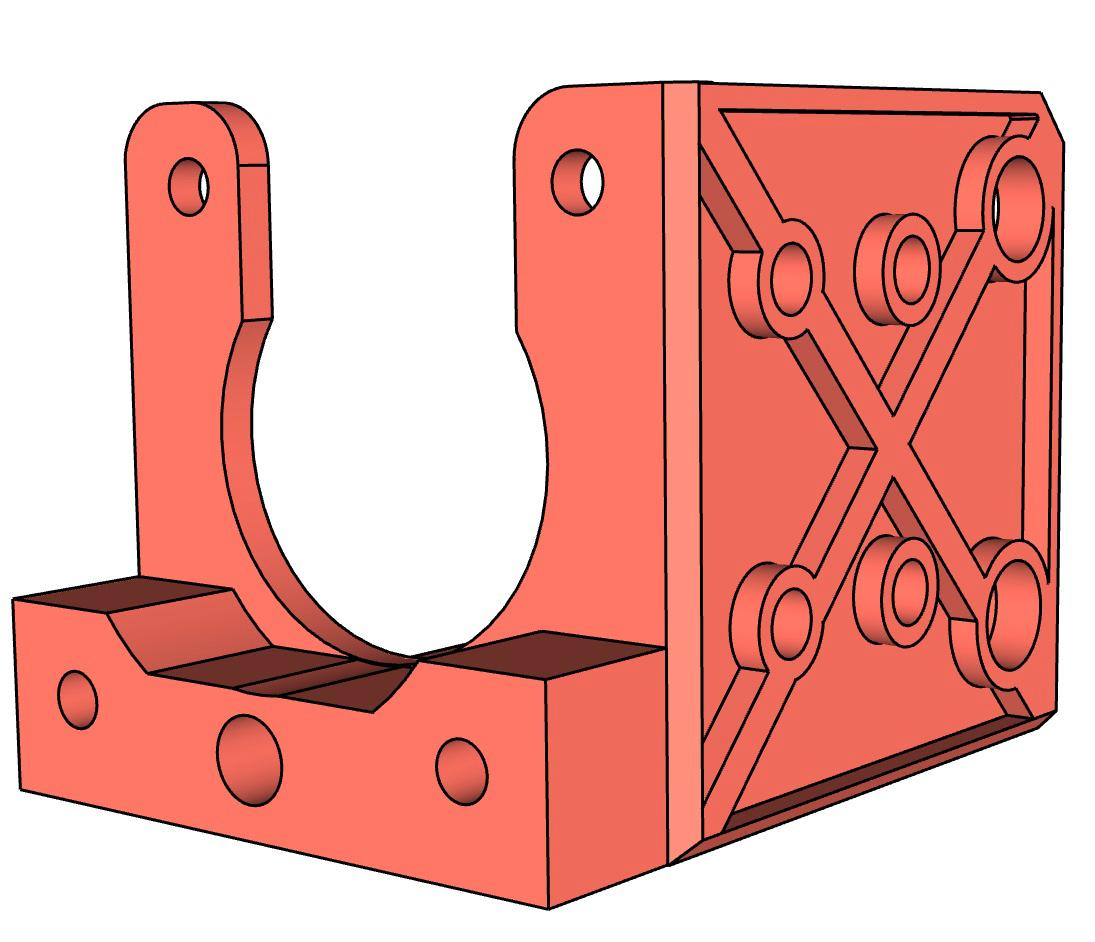
\includegraphics[scale = 0.4]{figuras/ressuportemotorhorizontalf}
\end{figure}
        
\begin{figure}[H]
\centering
\caption{Suporte do motor horizontal vista do verso.}\label{fig:ressuportemotorhorizontalfv}
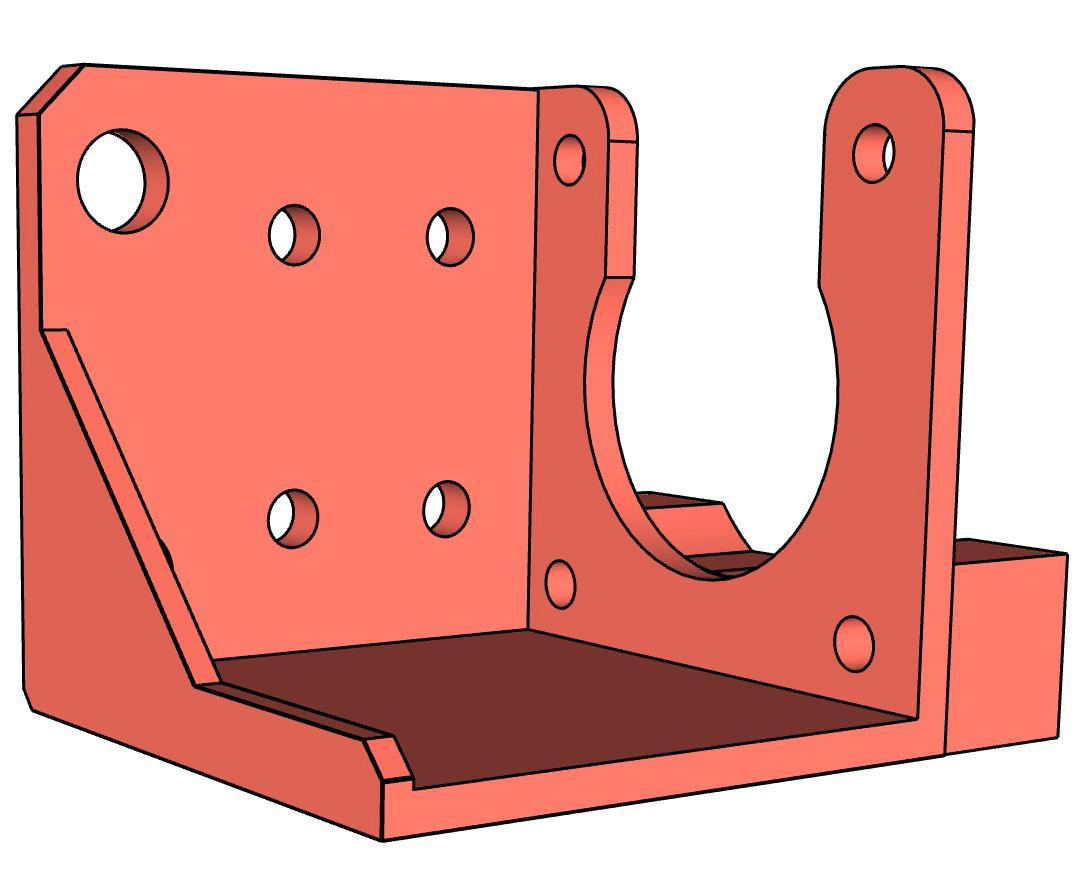
\includegraphics[scale = 0.4]{figuras/ressuportemotorhorizontalfv}
\end{figure}
        
\pagebreak

Para que este sistema se mantenha rígido, foi projetado o suporte que sustenta a outra 
extremidade do eixo e da haste, denominado de Suporte da Haste e do Mancal, também 
fabricado em \ac{PLA} conforme Figura \ref{fig:ressuportehastemancalf}. Nele foi fixado um 
mancal de rolamento, destinado a fixar o fuso, deixando-o livre para girar e também foi 
fixado um suporte em alumínio para sustentar a haste. Este suporte deve ser fixado a 
guia ajustável com roldanas.

\begin{figure}[H]
\centering
\caption{Suporte da haste e mancal vista da frente.}\label{fig:ressuportehastemancalf}
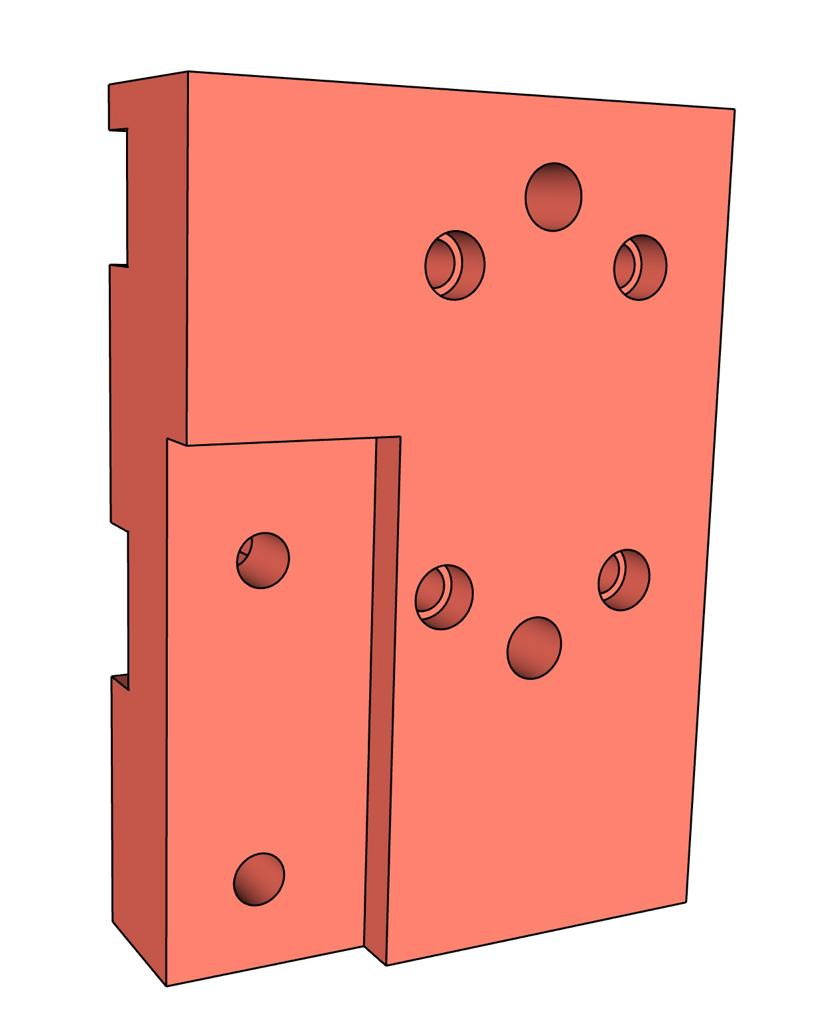
\includegraphics[scale = 0.4]{figuras/ressuportehastemancalf}
\end{figure}
    
\begin{figure}[H]
\centering
\caption{Suporte da haste e mancal vista do verso.}\label{fig:ressuportehastemancalfv}
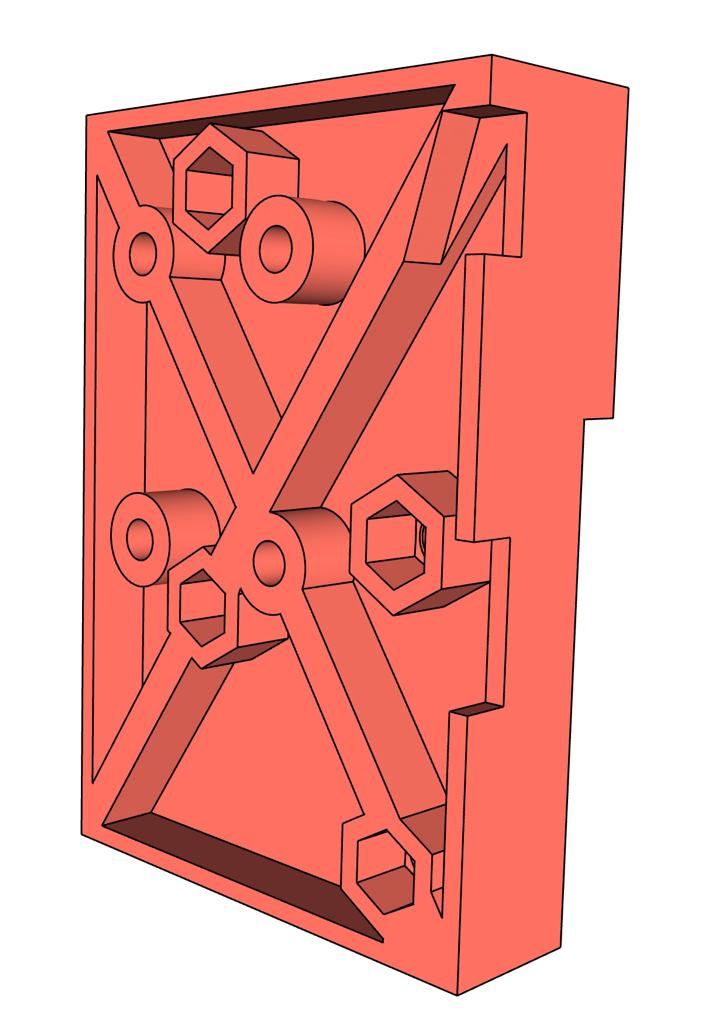
\includegraphics[scale = 0.4]{figuras/ressuportehastemancalfv}
\end{figure}

\pagebreak

Preso ao fuso e a haste temos o Suporte de serviço, assim denominado, pois é ele quem 
tem a função de segurar o tubo de Pitot e levá-lo a qualquer coordenada XY dentro 
da área útil de medição. Esse suporte é uma peça fabricada em \ac{PLA} e foi projetado 
em duas partes para facilitar sua montagem e se fixa ao fuso por meio de duas castanhas, 
que farão o deslocamento horizontal desse suporte. Para ampliar a área de medição 
desenvolveu-se um sistema que dá a opção de colocar o tubo de Pitot em cinco posições diferentes. 
Também foi levado em conta o volume da peça, como não requer muito esforço ela foi projetada 
em relevo para ficar mais leve.

\begin{figure}[H]
\centering
\caption{Suporte do serviço frontal vista da frente.}\label{fig:ressuporteservicofrontalf}
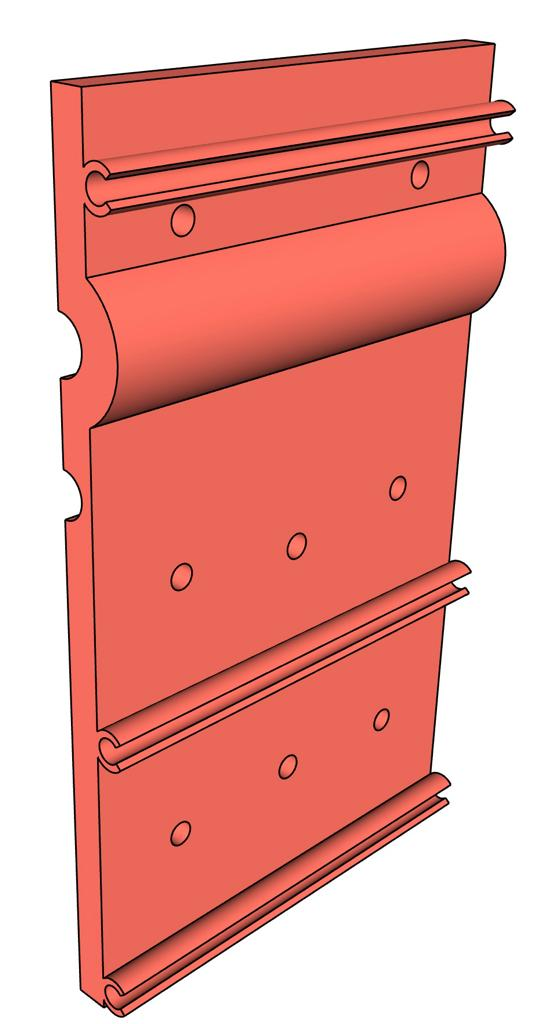
\includegraphics[scale = 0.4]{figuras/ressuporteservicofrontalf}
\end{figure}

\begin{figure}[H]
\centering
\caption{Suporte do serviço frontal vista do verso.}\label{fig:ressuporteservicofrontalfv}
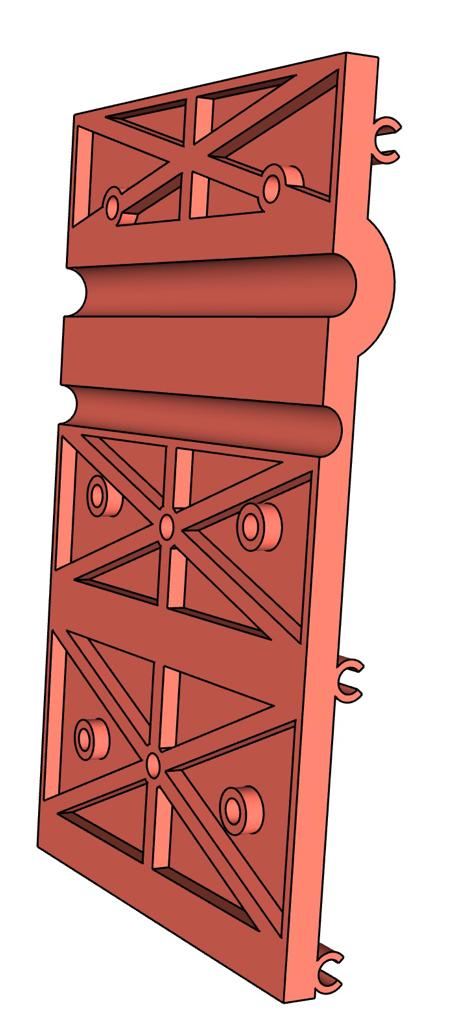
\includegraphics[scale = 0.4]{figuras/ressuporteservicofrontalfv}
\end{figure}
        
Todas as peças projetadas foram elaboradas com cuidado primeiramente em relação a aumentar 
a área de medição, que é de aproximadamente 500~x~463~mm, e depois com relação a montagem dos 
componentes, pois existem peças que obrigatoriamente devem ser montadas antes de outras. 

A seguir está a lista de materiais utilizados para a montagem da mesa cartesiana.

\begin{table}[H]
    \footnotesize
    \centering
    \caption{Lista de materiais.}
    \begin{tabular}{ll}
        \hline
        \textbf{Nome} & \textbf{Quantidade}\\
        \hline
        Perfil Estrutural em Aluminio 20~x~40~mm & 3,20~m\\
        Perfil Estrutural em Aluminio 20~x~20~mm & 0,5~m\\
        Conector Interno 90° com Parafusos p/ Perfil Base 20 V-Slot & 8~unidades\\
        Acoplamento Flexível em Alumínio 5~x~8~mm & 3~unidades\\
        Fuso Trapezoidal TR8~x~8~mm - 4 entradas & 1,3~m\\
        Eixo Linear em inox & 0,5~m\\
        Suporte SK em Alumínio para Eixo Linear Retificado e Inox & 1~unidade\\
        Mancal Modelo KP~8~mm & 3~unidades\\
        Placa de Conexão T p/ Perfil Base 20 V-Slot &2~unidades\\
        Guia Ajustável com Roldanas Para Perfil 20~x~40 V-Slot - 4~apoios & 2~unidades\\
        Placa para Perfil 20~x~20~mm em Alumínio Para Montagem V-Slot & 2~unidades\\
        Castanha em Latão p/Fuso Trapezoidal TR8~x~8~mm - 4~entradas & 4~unidades\\
        Parafuso Allen Cabeça Abaulada M6~x10~mm & 10~unidades\\
        Parafuso Allen Cabeça Abaulada M6~x16~mm & 8~unidades\\
        Parafuso Allen Cabeça Abaulada M5~x8~mm & 12~unidades\\
        Porca T Reforçada Canal 6 M6~Para V-Slot & 10~unidades\\
        Porca T Reforçada Canal 6 M5~Para V-Slot & 12~unidades\\
        \hline       
    \end{tabular}
    \label{tab:listamateriais}
\end{table}

\subsection{Discussão sobre os cálculos}

Será discutido os resultados dos cálculos situados na seção \ref{subsec:metcalculos}, 

De forma geral, os cálculos referentes as peças foram realizados de forma conservadora 
com o objetivo de serem dimensionados para a situação de maior carregamento.

Para a haste, foi estipulado uma deflexão máxima de $0,05~mm$ resultando em uma força de $22,92~N$ 
que equivale aproximadamente $2,3~kg$. Então, se comparar essa força ao peso da haste, que é de $619~g$ mais 
o peso do tubo de Pitot, que é de aproximadamente $80~g$ e o peso suporte de serviço, que é de aproximadamente 
$300~g$, se obtém aproximadamente $1~kg$. Sendo assim, a haste tem um fator de segurança de 2,3. 

\begin{itemize}
    \item massa específica ($\rho$) da haste é de $7,7~Mg/m^{3}$;
    \item volume da haste que tem como área, $2,010 \cdot 10^{-4}~m^{2}$ e comprimento de $0,4~m$, é de $8,04 \cdot 10^{-5}~m^{3}$;
    \item peso da haste de $619~g$. 
\end{itemize}

Para a parte do fuso calculou-se a força máxima que ele suportaria erguer, que é de 306,55~N ou 31,2~kg. 
Através dos cálculos realizados na seção \ref{subsec:metcalculos}. Encontrou-se o valor da tensão equivalente 
de Von Mises que é de 32,3~MPa.

Como o fabricante do fuso não especifica o aço utilizado na fabricação, foi considerado um aço inox~303, 
que é um dos aços com menor tensão de escoamento para validar o projeto. Considerando a tensão admissível 
do aço inox~303 que é de 241~MPa com a máxima tensão equivalente de Von Mises, encontrou-se um fator de 
segurança igual a 7,46. 

Através destes resultados, foi concluído que o peso do sistema junto aos equipamentos de medição estão bem 
abaixo dos valores máximos de forças e tensões suportados pelo sistema de transmissão.

%\section{Sistema eletrônico}\label{sec:ressisele}

\section{Sistema de software}\label{sec:ressissof}

O sistema de software do projeto foi fundamentado na metodologia, sendo assim para o desenvolvimento 
do código foi utilizado a plataforma de prototipação Arduino IDE respeitando o diagrama de classes 
mostrado na seção 3.3.3.

A seguir serão mostrados os arquivos header de cada classe presente no sistema a fim de resumir 
o código fonte da sua versão completa. Esta versão se encontra nos apêndices do trabalho.

%HEADER DA CLASSE PINO
\subsection{Código header da classe Pino}\label{subsec:respino}

Segue abaixo o arquivo header (Pino.h) da classe “Pino”.

{\lstinputlisting[
    language        = C++,
    morekeywords    = {Driver, Eixo, Pino, Sigmoidal},
    style           = mystyle
]{elementos-pos-textuais/apendices/Pinoh.txt}

%OBJETO DA CLASSE PINO
Assim para se utilizar as funções presentes na classe “Pino” é criado um objeto 
através do comando abaixo com seus devidos parâmetros de entrada.

\lstinputlisting[style = mystyle]{elementos-pos-textuais/apendices/Pinoobj.txt}

%HEADER DA CLASSE SIGMOIDAL
\subsection{Código header da classe Sigmoidal}\label{subsec:ressigmoidal}

Segue abaixo o arquivo header (Sigmoidal.h) da classe “Sigmoidal”.

\lstinputlisting[style = mystyle]{elementos-pos-textuais/apendices/Sigmoidalh.txt}

%OBJETO DA CLASSE SIGMOIDAL
Assim para se utilizar as funções presentes na classe “Sigmoidal” é criado um objeto 
através do comando abaixo com seus devidos parâmetros de entrada.

\lstinputlisting[style = mystyle]{elementos-pos-textuais/apendices/Sigmoidalobj.txt}

%HEADER DA CLASSE DRIVER
\subsection{Código header da classe Driver}\label{subsec:resdriver}
Segue abaixo o arquivo header (Driver.h) da classe “Driver”.

\lstinputlisting[style = mystyle]{elementos-pos-textuais/apendices/Driverh.txt}

%OBJETO DA CLASSE DRIVER
Para flexibilização na utilização de diferentes tipos de drivers, foi desenvolvido 
duas construções diferentes para utilizar as funções da classe “Driver”.

%OBJETO 1 CLASSE DRIVER
A primeira é passando como parâmetros o pino do passo e da direção como no código abaixo.
Essa construção é para drivers que se responsabilizam pelo controle do estado 
das bobinas através do seu hardware.

\lstinputlisting[style = mystyle]{elementos-pos-textuais/apendices/Driverobj.txt}

%OBJETO 2 CLASSE DRIVER
Já a segunda é passando como parâmetros os pinos das bobinas como no código abaixo.
Essa construção é para drivers que terceirizam para o software o controle
do estado das bobinas.

\lstinputlisting[style = mystyle]{elementos-pos-textuais/apendices/Driverobj2.txt}

%HEADER DA CLASSE EIXO
\subsection{Código header da classe Eixo}\label{subsec:reseixo}

Segue abaixo o arquivo header (Eixo.h) da classe “Eixo”.

\lstinputlisting[style = mystyle]{elementos-pos-textuais/apendices/Eixoh.txt}

%OBJETO DA CLASSE EIXO
Assim para se utilizar as funções presentes na classe “Eixo” é criado um objeto 
através do comando abaixo com seus devidos parâmetros de entrada.

\lstinputlisting[style = mystyle]{elementos-pos-textuais/apendices/Eixoobj.txt}

%EXPLICANDO COMO A MESACARTESIANA.INO FUNCIONA
\subsection{Detalhamento do arquivo principal (MesaCartesiana.ino)}\label{subsec:resmesa}

O arquivo principal tem a responsabilidade de gerenciar toda aplicação, neste arquivo 
foram construídos todos objetos necessários. Segue abaixo um resumo com todas 
funcionalidades que este possui.

\lstinputlisting[style = mystyle]{elementos-pos-textuais/apendices/MesaCartesianaino.txt}

O método “incializarEixos” é responsável por construir os objetos necessários para controle dos 
eixos da aplicação, neste é possível escolher se o tipo de acionamento do driver 
é via software ou hardware.

O método “interpretarComandos” é responsável pela interpretação de qual comando foi enviado pelo usuário,
como por exemplo o comando “MOVER 2,4” que movimenta o eixo X para a ordenada 2 e o eixo Y para a ordenada 4.
Outros comandos necessários para uma aplicação como a mudança de estados de algumas configurações 
devem ser interpretadas por este método.

O método “movimentarMesa” é responsável pela chamada da funcionalidade de rotação presente na classe “Eixo” 
para isso recebe como parâmetro a coordenada enviada pelo usuário.

O método “escolherModoPasso” é responsável por setar qual o modo do passo que o eixo irá operar.

O método “setup” é responsável pela inicialização de toda aplicação estando nele uma chamada 
para o método de inicialização dos eixos.

O método “serialEvent” é responsável pela recepção dos dados enviados pelo usuário estando nele uma chamada 
para o método de interpretação de comandos.

O método “loop” é responsável pela execução da aplicação de forma que ela nunca acabe, já que é necessário 
que o método “serialEvent” esteja sempre em operação para quando o usuário solicitar alguma ação no sistema 
esta seja executada.